\documentclass[a4paper]{article}
\usepackage[utf8]{inputenc}
\usepackage[spanish, es-tabla]{babel}

\usepackage[a4paper, footnotesep = 1cm, width=18cm, left=2cm, top=2.5cm, height=25cm, textwidth=18cm, textheight=25cm]{geometry}
%\geometry{showframe}

\usepackage{amsmath}
\usepackage{amsfonts}
\usepackage{amssymb}
\usepackage{float}
\usepackage{graphicx}
\usepackage{caption}
\usepackage{subcaption}
\usepackage{multicol}
\usepackage{multirow}
\setlength{\doublerulesep}{\arrayrulewidth}

\usepackage{hyperref}
\hypersetup{
    colorlinks=true,
    linkcolor=blue,
    filecolor=magenta,      
    urlcolor=blue,
    citecolor=blue,    
}

\newcommand{\quotes}[1]{``#1''}
\usepackage{array}
\newcolumntype{C}[1]{>{\centering\let\newline\\\arraybackslash\hspace{0pt}}m{#1}}
\usepackage[american]{circuitikz}
\usepackage{fancyhdr}
\usepackage{units} 

\pagestyle{fancy}
\fancyhf{}
\lhead{22.11 Electrónica I}
\rhead{Mechoulam, Lambertucci, Rodriguez, Londero}
\rfoot{Página \thepage}

\begin{document}

%%%%%%%%%%%%%%%%%%%%%%%%%
%		Caratula		%
%%%%%%%%%%%%%%%%%%%%%%%%%

\begin{titlepage}
\newcommand{\HRule}{\rule{\linewidth}{0.5mm}}
\center
\mbox{\textsc{\LARGE \bfseries {Instituto Tecnológico de Buenos Aires}}}\\[1.5cm]
\textsc{\Large 22.11 Electrónica I}\\[0.5cm]


\HRule \\[0.6cm]
{ \Huge \bfseries Trabajo práctico N$^{\circ}$1}\\[0.4cm] 
\HRule \\[1.5cm]


{\large

\emph{Grupo 3}\\
\vspace{3px}

\begin{tabular}{lr} 	
\textsc{Mechoulam}, Alan  &  58438\\
\textsc{Lambertucci}, Guido Enrique  & 58009 \\
\textsc{Rodriguez Turco}, Martín Sebastian  & 56629 \\
\textsc{Londero Bonaparte}, Tomás Guillermo  & 58150 \\
\end{tabular}

\vspace{20px}

\emph{Profesores}\\
Alcocer, Fernando\\
Oreglia, Eduardo Victor\\
Gardella, Pablo Jesús\\
\vspace{3px}
%\textsc{} \\	

\vspace{100px}

\begin{tabular}{ll}

Presentado: & 24/09/19\\

\end{tabular}

}

\vfill

\end{titlepage}


%%%%%%%%%%%%%%%%%%%%%
%		Indice		%
%%%%%%%%%%%%%%%%%%%%%

\tableofcontents
\newpage

%%%%%%%%%%%%%%%%%%%%%
%		Informe		%
%%%%%%%%%%%%%%%%%%%%%
\section{Introducción}
En el siguiente informe se busca analizar, desarrollar y confeccionar algún circuito estudiado a lo largo del cuatrimestre. Se destaca la existencia de una dificultad adicional, la cual se basa en el método mediante el cual se fueron adquiriendo los componentes. Estos fueron subastados durante la cursada, entre los diversos grupos. De esta forma, se condiciona el circuito final, ya que se posee acceso limitado a estos, los cuales no se pudieron elegir libremente.

\section{Desarrollo}

\subsection{Componentes dispuestos}
El presente grupo se valió de los siguientes componentes:
\begin{itemize}
	\item Dos pares de resistencias de $6.8 \ k\Omega$ y de $680 \ k\Omega$.
	\item Un transistor BJT NPN. 
	\item Un diodo 1N4148.
	\item Un JFET.
	\item Un par Darlington NPN.
	\item Una placa de 5x5.
\end{itemize}

\subsection{Circuitos considerados}
Como primer opción se consideró utilizar el par Darlington y mediante el uso de las resistencias, configurarlo de forma tal que este quede compensado. Una alternativa es el uso de una fuente de corriente, con el mismo objetivo que se mencionó anteriormente.
\begin{figure}[H]
\centering
\begin{subfigure}{.45\textwidth}
\centering
	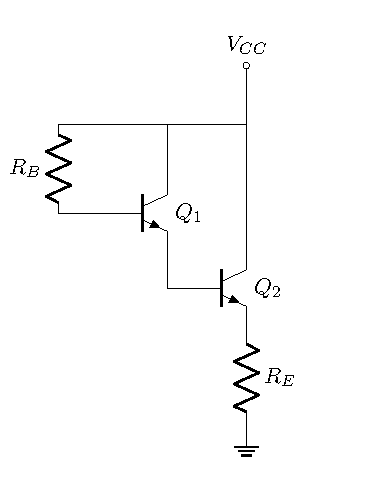
\includegraphics[width=0.5\textwidth, page=1]{Imagenes/ParDarlington.pdf}
	\caption{Par Darlington.}
	\label{fig:pardar1}
\end{subfigure}
\begin{subfigure}{.4\textwidth}
\centering
	\includegraphics[width=0.6\textwidth, page=2]{Imagenes/ParDarlington.pdf}
	\caption{Par Darlington compensado con $R$.}
	\label{fig:pardar2}
\end{subfigure}
\begin{subfigure}{.5\textwidth}
\centering
	\includegraphics[width=0.5\textwidth, page=3]{Imagenes/ParDarlington.pdf}
	\caption{Par Darlington compensado con fuente de corriente.}
	\label{fig:pardar3}
\end{subfigure}
\caption{Configuraciones posibles para el par Darlington.}
\label{fig:pardar}
\end{figure}

La conexión representada en la Figura (\ref{fig:pardar1}) no es conveniente, ya que la caída de tensión entre la base y el emisor se encuentra entre $0.6 \ V$ y $1.5 \ V$, siendo esta resultante de la suma de las tensiones base-emisor de ambos transistores. Esto genera a su vez que el dispositivo consuma más corriente y aumente su temperatura, además de generar respuestas más lentas frente a cambios en la entrada. Una solución a lo ya expresado se presenta en la Figura (\ref{fig:pardar2}).

Estrictamente hablando, esta disposición es la más económica al problema anterior. Dadas las condiciones, dicha consideración no afecta en la decisión a implementar, ya que se cuenta con componentes para realizar cualquiera de las tres. Finalmente, la mostrada en la Figura (\ref{fig:pardar3}) es más optima para compensar el circuito, ya que permite aumentar $I_{CEQ}$ sin modificar otros factores del propio circuito.

Se puede colocar un diodo entre el colector y el emisor de $Q_2$. Este tipo de configuración es utilizada para trabajar con potencias altas. Dado que este enfoque no es de interés, se reserva dicho componente.

\subsection{Fuente de corriente}
\label{subsec:fdei}
Una vez determinado que la implementación optima, con los componentes disponibles, es la presentada en la Figura~(\ref{fig:pardar3}), se decide confeccionarla. Para ello, primero se opta por analizar la fuente de corriente. Esta puede ser realizada con el JFET, dispuesto en una configuración en la cual se autopolarice, como se presenta a continuación.
\begin{figure}[H]
\centering
	\includegraphics[width=0.25\textwidth, page=4]{Imagenes/ParDarlington.pdf}
	\caption{Fuente de corriente.}
	\label{fig:fuentei}
\end{figure}

Recorriendo la malla de entrada y de salida del circuito de la Figura (\ref{fig:fuentei}), se obtienen las siguientes ecuaciones:
\begin{equation}
	V_{GS} = V_{SS} - I_{DS} R_{S}
\end{equation}
\begin{equation}
	V_{DS} = V_{DD} + V_{SS} - I_{DS} \left( R_{D} + R_{S} \right)
\end{equation}

Además, se plantean las ecuaciones del JFET:
\begin{equation}
\begin{split}
	I_{DS} = I_{DSS} & \left( 1 - \frac{V_{GS}}{V_P} \right)^2 \\
	gm = & \ 2\frac{\sqrt{I_{DS} I_{DSS}}}{|V_P|}
\end{split}
\end{equation}

De esta forma, seleccionando el componente \href{https://www.onsemi.com/pub/Collateral/2N3819-D.PDF}{2N3819}, se obtiene de la hoja de datos los valores de interés, tales como $I_{DSS} = 2 \ mA$ y $V_P = -8 \ V$ (para el peor caso). Luego, estableciendo $V_{SS} = 10 \ V$, $R_S = 6.8 \ K\Omega$ y $R_D = 680 \ \Omega$ se calculan la corriente de drain y la tensión gate-source. Como es de esperarse, se obtienen dos valores posibles para cada variable:

%\begin{equation*}
%I_{DS} = \left\lbrace
%\begin{split}
%	& 4.39 \ mA \\
%	& 1.60 \ mA
%\end{split}
%\right.
%\ \ \
%V_{GS} = \left\lbrace
%\begin{split}
%	& -19.85 \ V \\
%	& -0.88 \ V
%\end{split}
%\right.
%\end{equation*}

\begin{equation*}
\left\lbrace
\begin{split}
	&I_{DS} =  4.39 \ mA \\
	&V_{GS} =  -19.85 \ V
\end{split}
\right.
\ \ y \ \
\left\lbrace
\begin{split}
	&I_{DS} =  1.60 \ mA \\
	&V_{GS} =  -0.88 \ V
\end{split}
\right.
\end{equation*}

Sabiendo que se debe cumplir que $I_{DSS} \geq I_{DS}$ y $V_{GS} > V_{P}$, se descartan los primeros valores, seleccionando $I_{DS} = 1.60 \ mA$ y $V_{GS} = -0.88 \ V$, obteniéndose así $gm = 0.45 \ \frac{mA}{V}$. De esta forma se garantiza que esté polarizado adecuadamente. \textcolor{red}{Por otro lado, para garantizar que se cumpla $V_{DS} > V_{DSE} = |V_{GS} - V_P|$, se requiere el valor de $V_{DD}$. Dado que este circuito es empleado para polarizar otro, dicha tensión queda fijada por la totalidad del circuito, por lo que este análisis es expuesto más adelante.}  
% http://www2.eng.cam.ac.uk/~dmh/ptialcd/jfet/2N3819.pdf https://www.mouser.com/datasheet/2/149/2n3819-286408.pdf
%Por otro lado, $V_{DD}$ queda fijado por el circuito del Darlington, siendo esta $V_{DD} = V_{BEON} = 0.7 \ V$.

Con lo establecido previamente, se prosigue a plantear el circuito incremental. Es de interés calcular la impedancia de salida, para luego emplearla para calcular las variables pertinentes en el circuito de la Figura (\ref{fig:pardar3}).
\begin{figure}[H]
\centering
	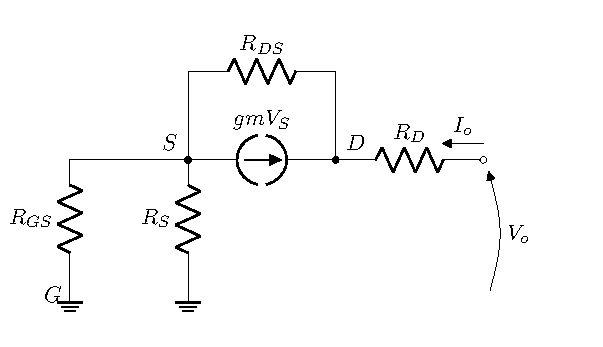
\includegraphics[width=0.45\textwidth, page=1]{Imagenes/ModeloIncremental.pdf}
	\caption{Circuito incremental de la Figura (\ref{fig:fuentei}).}
\label{fig:incfuente1}
\end{figure}

Se destaca que, como el gate queda a tierra, se cumple que $V_{GS} = V_G - V_S = - V_S$, por lo tanto, se da vuelta la fuente de corriente y se reemplaza con lo mencionado anteriormente. 

Se define $R_S^* = R_S // R_{GS}$, para luego analizar el circuito presentado en la Figura (\ref{fig:incfuente2}).
\begin{figure}[H]
\centering
\hspace*{2cm}
	\includegraphics[width=0.4\textwidth, page=2]{Imagenes/ModeloIncremental.pdf}
	\caption{Análisis de la impedancia de salida del circuito de la fuente de corriente.}
\label{fig:incfuente2}
\end{figure}

Planteando la tensión $V_o$ y las corrientes del nodo $D$, se obtienen las siguientes expresiones respectivamente.
\begin{equation*}
	V_o = I_{DS} R_{DS} + I_o \left( R_D + R_S^* \right)
\end{equation*}
\begin{equation*}
	I_{DS} = gm V_S + I_o = \left( gm R_S^* + 1 \right) I_o
\end{equation*}

Operando algebraicamente se obtiene la variable deseada de la forma:
\begin{equation}
\begin{split}
	R_{OF} & = \frac{V_o}{I_o} = R_{DS} \left( 1 + gm R_S^* \right) + R_S^* + R_D \\
		   & = R_{DS} \left( 1 + gm R_S//R_{GS} \right) + R_S//R_{GS} + R_D
\end{split}
\label{equ:rof}
\end{equation}

Para poder continuar, se toma $R_{GS} \longrightarrow \infty$, luego se asume $V_A = -90 \ V$, estimando así $R_{DS} = \frac{V_A}{I_{DS}} = 56.25 \ K\Omega$. De esta forma se obtiene de (\ref{equ:rof}) el valor de la impedancia de salida $R_{OF} \approx 240.91 \ K\Omega$.

\subsection{Darlington polarizado por corriente}
Con lo obtenido en la Sección (\ref{subsec:fdei}), se posee la información necesaria para analizar el circuito presentado en la Figura (\ref{fig:pardar3}). El primer paso, consiste en reemplazar la fuente de corriente por su respectiva impedancia de salida $R_{OF}$. En el análisis que se muestra a continuación se presentan la carga y la alimentación del sistema, componentes que no fueron presentados en la Figura (\ref{fig:pardar}) por cuestiones de simplicidad.
\begin{figure}[H]
\centering
	\includegraphics[width=0.5\textwidth, page=5]{Imagenes/ParDarlington.pdf}
	\caption{Circuito equivalente al reemplazar la fuente de corriente.}
	\label{fig:pardar4}
\end{figure}

De manera análoga al análisis presentado para la fuente de corriente, se parte por la polarización. Primero se establecen $V_{CC} = 15 \ V$, $R_C = 6.8 \ K\Omega$ y $R_B = 680 \ \Omega$. Como se está polarizando $Q_1$ con una fuente de corriente, queda definido que $I_{CE1} = I_{DS} = 1.60 \ mA$.

Por otro lado, para el transistor $Q_2$ se plantea
\begin{equation*}
	V_{CC} - 2 V_{BEON} = I_{CE2} R_{C}
\end{equation*}
\begin{equation}
	I_{CE2} = \frac{V_{CC} - 2 V_{BEON}}{R_{C}} = 2 \ mA
\end{equation}

Habiendo establecido esto, se puede calcular $V_{CE1}$ y $V_{CE2}$ de la forma
\begin{equation*}
	V_{CE1} = V_{CC} - V_{BEON} - I_{CE2} R_{C} = 0.7 \ V
\end{equation*}
\begin{equation}
	V_{CE2} = V_{CC} - I_{CE2} R_{C} = 1.4 \ V
\end{equation}

\begin{center}
	\LARGE{\textcolor{red}{\textbf{VERIFICAR POLARIZACIÓN.}}}
\end{center}

Se decidió seleccionar transistores \href{https://www.sparkfun.com/datasheets/Components/BC546.pdf}{BC547} para este par, tomando $h_{FE1} = h_{FE2} = h_{FE} = 110$ de la hoja de datos. Es así que se procede al modelo incremental, asumiendo $T = 27^o C$ y $V_{A1} = V_{A2} = V_A = -90 \ V$, y sabiendo que los estimadores empleados son $gm = \frac{I_{CE}}{V_T}$, $h_{ie} = \frac{h_{fe}}{gm}$ y $\frac{1}{h_{o1}} = \frac{V_A}{I_{CE}}$, se consiguen los siguientes valores:
\begin{table}[H]
\centering
\begin{tabular}{cccc}
\hline
\textbf{Transistor} & $\mathbf{gm \ \left[ \frac{mA}{V} \right]}$ & $\mathbf{h_{ie} \ \left[ K\Omega \right]}$ & $\mathbf{\frac{1}{h_{oe}} \ \left[ K\Omega \right]}$ \\
\hline
$Q_1$ & 61.89 & 1.78 & 56.25 \\
$Q_2$ & 77.36 & 1.42 & 45	\\
\hline
\end{tabular}
\caption{Estimadores del modelo incremental del circuito Darlington.}
\label{tab:estim}
\end{table}

Planteando su respectivo modelo incremental, se llega al circuito presentado a continuación: 
\begin{figure}[H]
\centering
	\includegraphics[width=0.85\textwidth, page=3]{Imagenes/ModeloIncremental.pdf}
	\caption{Modelo incremental del par Darlington.}
\label{fig:incdar}
\end{figure}

Definiéndose $R_{OF}^* = R_{OF} // \frac{1}{h_{oe1}}$ y $R_d = R_C // \frac{1}{h_{oe2}} // R_L$, se obtiene
\begin{figure}[H]
\centering
	\includegraphics[width=0.8\textwidth, page=4]{Imagenes/ModeloIncremental.pdf}
\end{figure}

Donde $I_{B1}^* = I_{B1} \left( 1 + h_{fe1} \right)$ y $I_{B2}^* = I_{B2} \left( 1 + h_{fe2} \right)$. Aplicando paso a nivel de corriente se llega a
\begin{figure}[H]
\centering
	\includegraphics[width=0.8\textwidth, page=5]{Imagenes/ModeloIncremental.pdf}
\end{figure}

Por un lado se destaca que 
\begin{equation*}
	V_o = I_{B2} R_d \left( 1 + h_{fe2} \right)
\end{equation*}

Siendo así
\begin{equation}
	\frac{V_o}{I_{B2}} = R_d \left( 1 + h_{fe2} \right)
\label{equ:vo-ib2}
\end{equation}

Por otro lado, se analiza la relación entre $I_{B1}^*$ e $I_{B2}^*$ mediante un divisor de corrientes, consiguiéndose
\begin{equation*}
	I_{B2} = I_{B1}^* \frac{R_{OF}^*}{R_{OF}^* + h_{ie2} + R_d \left( 1 + h_{fe2} \right)} = I_{B1} \frac{R_{OF}^* \left( 1 + h_{fe1} \right)}{R_{OF}^* + h_{ie2} + R_d \left( 1 + h_{fe2} \right)}
\end{equation*}

Dividiéndose a ambos lados por $I_{B1}$
\begin{equation}
	\frac{I_{B2}}{I_{B1}} = \frac{R_{OF}^* \left( 1 + h_{fe1} \right)}{R_{OF}^* + h_{ie2} + R_d \left( 1 + h_{fe2} \right)} 
\label{equ:ib2-ib1}
\end{equation}

Luego, se observa que
\begin{equation}
	V_i = I_{B1} h_{ie1} + I_{B2} \left[ h_{ie2} + R_d \left( 1 + h_{fe2} \right) \right]
\label{equ:vi-ib1-ib2}
\end{equation}

Utilizando (\ref{equ:ib2-ib1}) en (\ref{equ:vi-ib1-ib2}), se llega a la expresión
\begin{equation}
	\frac{V_i}{I_{B1}} =  h_{ie1} + \frac{ R_{OF}^* \left[ h_{ie2} + R_d \left( 1 + h_{fe2} \right) \right] \left( 1 + h_{fe1} \right)}{R_{OF}^* + h_{ie2} + R_d \left( 1 + h_{fe2} \right)}
\label{equ:vi-ib1}
\end{equation}

Con lo obtenido en (\ref{equ:vo-ib2}), (\ref{equ:ib2-ib1}) y (\ref{equ:vi-ib1}), se procede a calcular la transferencia $\Delta V$, siendo esta de la forma
\begin{equation}
\begin{split}
	\Delta V \triangleq \frac{V_o}{V_i} = \frac{V_o}{I_{B2}} \frac{I_{B2}}{I_{B1}} \frac{I_{B1}}{V_i} = \frac {R_d R_{OF}^* \left( 1+h_{fe2} \right) \left( 1+h_{fe1} \right) }{ \left[ R_d \left( 1+h_{fe2} \right) \left( 1+h_{fe1} \right) +h_{fe1}h_{ie2}+h_{ie1}+h_{ie2} \right] R_{OF}^*+h_{ie1} \left[ h_{ie2}+R_d \left( 1+h_{fe2} \right)  \right] }
\end{split}
\label{equ:v}
\end{equation}

Para la ganancia de corriente se observa nuevamente la Figura (\ref{fig:incdar}). Aplicando un divisor de corriente a la salida se obtiene una expresión que relaciona $I_{B2}$ con $I_o$.
\begin{equation*}
	I_o = I_{B2} \left( 1 + h_{fe2} \right) \frac{R_C // \frac{1}{h_{oe2}}}{R_C // \frac{1}{h_{oe2}} + R_L}
\end{equation*}
\begin{equation}
	\frac{I_o}{I_{B2}} = \left( 1 + h_{fe2} \right) \frac{R_C // \frac{1}{h_{oe2}}}{R_C // \frac{1}{h_{oe2}} + R_L}
	\label{equ:io-ib2}
\end{equation}

Luego, se plantean las corrientes para el nodo $B_1$.
\begin{equation*}
	I_i = \frac{V_i}{R_B} + I_{B1}
\end{equation*}
\begin{equation}
	\frac{I_i}{I_{B1}} = 1 + \frac{V_i}{I_{B1}} \frac{1}{R_B}
\label{equ:ii-ib1}
\end{equation}

Por lo tanto, de la misma forma que se realizó para la ganancia de tensión, mediante el uso de (\ref{equ:ib2-ib1}), (\ref{equ:vi-ib1}), (\ref{equ:io-ib2}) y (\ref{equ:ii-ib1}), se calcula la ganancia de corriente.
\begin{equation*}
	\Delta I \triangleq \frac{I_o}{I_i} = \frac{I_o}{I_{B2}} \frac{I_{B2}}{I_{B1}} \frac{I_{B1}}{I_i}
\end{equation*}
\begin{equation}
	\Delta I = \frac { R_C R_{OF}^* R_B \left( 1+h_{fe2} \right) \left( 1+h_{fe1} \right)}{D}
\end{equation}

Siendo
\begin{equation}
\begin{split}
D = & \left( R_C R_L h_{oe2}+R_C+R_L \right)  \left\lbrace \left[ h_{ie2} + R_d \left( 1+h_{fe2} \right) \right] \left( R_B+h_{ie1} \right) + \right. \\
& \left. \left[ R_d \left( 1+h_{fe2} \right)  \left( 1+h_{fe1} \right) + h_{fe1} h_{ie2} + R_B + h_{ie1} + h_{ie2} \right] R_{OF}^* \right\rbrace
\end{split}
\end{equation}

A continuación, se calcula la impedancia de entrada del amplificador, mediante el uso de (\ref{equ:vi-ib1}) y (\ref{equ:ii-ib1}), siendo esta
\begin{equation*}
	R_{ia} = \frac{V_i}{I_i} =  \frac{V_i}{I_{B1}}\frac{I_{B1}}{I_i}
\end{equation*}
\begin{equation}
R_{ia} = \frac{\left\lbrace  \left[ R_{d} \left( 1+h_{fe2} \right) \left( 1+h_{fe1} \right) + h_{fe1}h_{ie2} + h_{ie1} + h_{ie2} \right] R_{OF}^* + h_{ie1} \left[ h_{ie2} + R_{d} \left( 1 + h_{fe2} \right) \right] \right\rbrace R_{B}}{\left[ R_{d} \left( 1+h_{fe2} \right) \left( 1 + h_{fe1} \right) + h_{ie1} + \left( 1 + h_{fe1} \right) h_{ie2} + R_{B} \right] R_{OF}^* + \left[ h_{ie2} + R_{d} \left( 1 + h_{fe2} \right) \right] \left( R_{B} + h_{ie1} \right)}
\end{equation}

Por otro lado, para el calculo de la impedancia de salida $R_{oa}$ se considera el circuito de la siguiente forma:
\begin{figure}[H]
\centering
	\includegraphics[width=0.8\textwidth, page=6]{Imagenes/ModeloIncremental.pdf}
\end{figure}
Se definen $R_{S}^* = \left( R_B // R_S \right) + h_{ie1}$ y $R_C^* = R_C // \frac{1}{h_{oe1}}$. Luego, sabiendo que la tensión sobre $R_{OF}^*$ y $R_{S}^*$ es la misma, se obtiene
\begin{equation}
	I_{OF} = I_{B1} \frac{R_{S}^*}{R_{OF}^*}
	\label{equ:roa1}
\end{equation}

Luego, observando el nodo $E_2$, se llega a
\begin{equation}
	I_{B2} \left( 1 + h_{fe2} \right) + I_o = \frac{V_o}{R_{C}^*}
	\label{equ:roa2}
\end{equation}

Se expresa la tensión $V_o$ como
\begin{equation}
	V_o = - \left( I_{B1} h_{ie1} + I_{B2} h_{ie2} \right)
	\label{equ:roa3}
\end{equation}
y se plantea para el nodo $C_1$, utilizando (\ref{equ:roa1}), llegándose a la expresión
\begin{equation}
	I_{B1} \left( 1 + h_{fe1} \right) + I_{OF} + I_{B2} h_{ie2} + I_o = \frac{V_o}{R_{C}^*}
	\label{equ:roa4}
\end{equation}

De esta forma, con (\ref{equ:roa2}), (\ref{equ:roa3}) y (\ref{equ:roa4}), se opera algebraicamente y se obtiene finalmente la impedancia de salida del circuito
\begin{equation}
R_{oa} = \frac{V_o}{I_o} = 
\frac {R_{C}^* \left[ \left( h_{fe1} + 1 \right) R_{OF}^* + R_{S}^* \right] \left( 1 + h_{fe2} \right) }{ \left[ \left( h_{ie2} R_{C}^* + 3 h_{fe2} + 3 \right) h_{fe1} + h_{ie2} R_{C}^* + h_{fe2} + 1 \right] R_{OF}^* + \left( h_{ie2} R_{C}^* + h_{fe2} + 1 \right) R_{S}^* }
\end{equation}

Una vez calculada $\Delta V$, $\Delta I$ y $R_{ia}$, se puede calcular la ganancia de tensión del sistema $\Delta V_S$, siendo esta
\begin{equation}
\begin{split}
	\Delta V_S \triangleq \frac{V_S}{V_i} = \frac{V_S}{V_o} \frac{V_o}{V_i} = \frac{V_o}{V_i} \frac{R_i}{R_S + R_{ia}}
\end{split}
\label{equ:vs}
\end{equation}

\subsection{Desarrollo y armado de la placa}
\begin{center}
	\LARGE{\textcolor{red}{\textbf{Esquemático, PCB y foto.}}}\\
	\LARGE{\textcolor{red}{\textbf{Consideraciones necesarias para medir.}}}
\end{center}

\subsection{Mediciones}

\section{Conclusiones}
Dado que se optó por confeccionar una configuración Darlington, se puede afirmar que la ganancia de corriente del circuito, la cual ya de por sí es grande, como se demostró en \textcolor{red}{\textbf{(...)}}, es mayor que la de los demás grupos, ya que la principal característica de este es la alta ganancia de dicha variable. Por otro lado, también es posible afirmar que la polarización resulta altamente estable, ya que se logró efectuar la polarización mediante una fuente de corriente.
	
\end{document}